\subsection{Second problem}

\begin{figure}[H]
    \centering    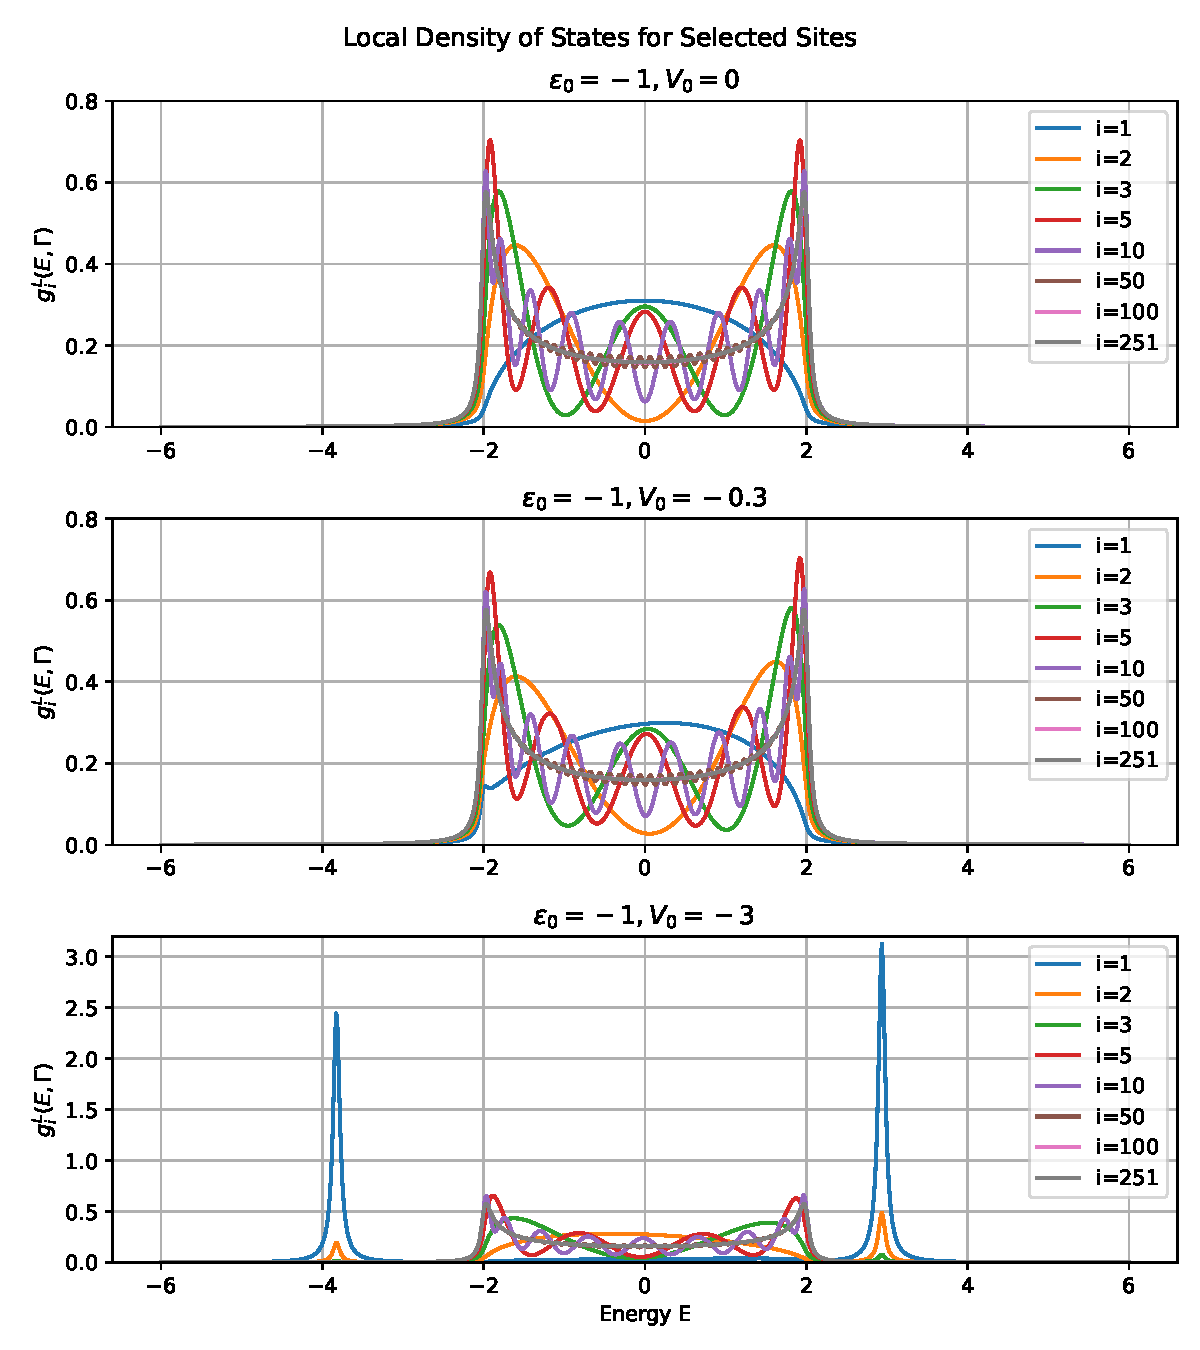
\includegraphics[width=\textwidth]{Figures/task2.pdf}
    \caption{LDOS plotted for a 1D chain of length $N=501$ with surface at site $i=1$ and adsorbate at site $i=0$. The index $i$ corresponds to the site number in the chain.}
    \label{fig:task2}
\end{figure}

\textbf{A2} For the first case, the top plot in Fig. \ref{fig:task2}, The LDOS is the same for all sites as in task 1, except at the site $i=0$. That is, the adsorbate atom. This is reasonable since there is no coupling between the adsorbate and the chain since $V_0 = 0$. For the second case, the middle plot in Fig. \ref{fig:task2}, there is some coupling between the adsorbate and the chain which is mainly noticeable at sites close to the adsorbate. At energy approximately $-2$ the LDOS is lower for site $i=1$, so the adsorbate occupies some possible modes for the first atom in the chain. However, most of the other sites are barely unaffected. The effect is hard to see beyond site $i=3$. For the last case, the bottom plot in Fig. \ref{fig:task2}, the adsorbate has a much higher coupling of $V_0 = -3$ and is clearly affecting the chain. The sites closest to the adsorbate have modes considerably lower and higher than they had without the adsorbate. However, at site $i=10$ it is hard to see the effect of the adsorbate. The adsorbate is clearly affecting the atoms closest to it, but it not only the nearest neighbour atom, even though it only has a coupling to that one.

It is also clear that for the adsorbate the LDOS is centred around a lower energy as the coupling potential decreases. The spike is of the LDOS is also much sharper for a stronger coupling. It looks like when the coupling is strong the chain closest to the adsorbate is almost decoupled from the rest of the chain and behaves more like the adsorbate itself than the other atoms in the chain.